\section{Resultados}

Los resultados de esta secci\'on corresponden a las ejecuciones MATLAB R2025a registradas en \texttt{simulacion/pruebas/reporte\_validacion.json}. Los par\'ametros de CPU y GPU son hip\'otesis de simulaci\'on; las temperaturas que siguen son resultados calculados para el modelo idealizado y no mediciones de una computadora.

\subsection{Escenario base y comparaci\'on de solucionadores (objetivos i, ii y iv)}

En la malla base de $49\times33$ nodos, el campo directo disperso alcanz\'o $T_{\max}=77.7592\ ^\circ$C en $(x,y)=(0.175,0.100)$ m, dentro de la huella GPU. El borde conserv\'o exactamente $25\ ^\circ$C. La cuadratura de las fuentes materializ\'o $12$ W en CPU y $18$ W en GPU, para un total discreto de $30$ W. El mapa de la Figura~\ref{fig:mapa-termico} mostr\'o dos regiones calientes, con un m\'aximo global junto a la fuente de mayor potencia.

La Tabla~\ref{tab:base-solver} compar\'o los m\'etodos con la misma matriz, vector, tolerancia $10^{-8}$ y condici\'on inicial. Ambos m\'etodos iterativos convergieron; CG necesit\'o 127 iteraciones frente a 2145 de Gauss--Seidel. Sus temperaturas m\'aximas difirieron de la referencia directa en menos de $8\times10^{-6}\ ^\circ$C. El residuo directo fue $3.69\times10^{-15}$. Como indicador complementario, GS termin\'o con $E_k=1.05\times10^{-9}$; la parada sigui\'o determinada por el residuo relativo. La Figura~\ref{fig:residuos} present\'o el historial: CG alcanz\'o la tolerancia en muchas menos iteraciones. Los tiempos se midieron con una corrida de calentamiento y tres repeticiones por configuraci\'on; se informa la mediana y su dispersi\'on.

La Figura~\ref{fig:aproximaciones} compara el campo reconstruido en el estado inicial, en una iteraci\'on intermedia y al converger. Para cada m\'etodo, el estado inicial corresponde a $k=0$ y es uniforme a $25\ ^\circ$C; los estados intermedios se guardaron al alcanzar aproximadamente la mitad del n\'umero de iteraciones convergidas: $k=1073$ para Gauss--Seidel y $k=64$ para CG. En ambos paneles finales se usan los resultados de las corridas can\'onicas, con $k=2145$ y $k=127$, respectivamente. La escala crom\'atica com\'un permite comparar los campos sin cambiar el rango de temperatura entre paneles.

\begin{table}[t]
\centering
\begin{threeparttable}
\caption{Soluci\'on del escenario base en la malla $49\times33$}
\label{tab:base-solver}
\scriptsize
\setlength{\tabcolsep}{3pt}
\begin{tabular}{lrrrr}
\toprule
M\'etodo & Iter. & Residuo & $T_{\max}$ ($^\circ$C) & Mediana (s)\\
\midrule
Directo disperso & 1 & $3.69\times10^{-15}$ & 77.759239 & 0.00324\\
Gauss--Seidel & 2145 & $9.94\times10^{-9}$ & 77.759232 & 0.20536\\
Gradiente Conjugado & 127 & $9.28\times10^{-9}$ & 77.759239 & 0.00482\\
\bottomrule
\end{tabular}
\begin{tablenotes}\footnotesize
\item \textit{Nota.} La tolerancia de los m\'etodos iterativos es $10^{-8}$. Cada mediana resume tres repeticiones, tras una corrida de calentamiento; las desviaciones est\'andar de esta reproducci\'on fueron $0.00542$ s (Gauss--Seidel), $0.000258$ s (CG) y $0.000229$ s (directo). Los tiempos cambiaron frente a la ejecuci\'on registrada anteriormente y dependen del equipo y de la carga del sistema. El error m\'aximo entre el campo iterativo y la referencia fue $1.17\times10^{-5}\ ^\circ$C para Gauss--Seidel y $4.93\times10^{-7}\ ^\circ$C para CG.
\end{tablenotes}
\end{threeparttable}
\end{table}

\begin{figure}[t]
\centering
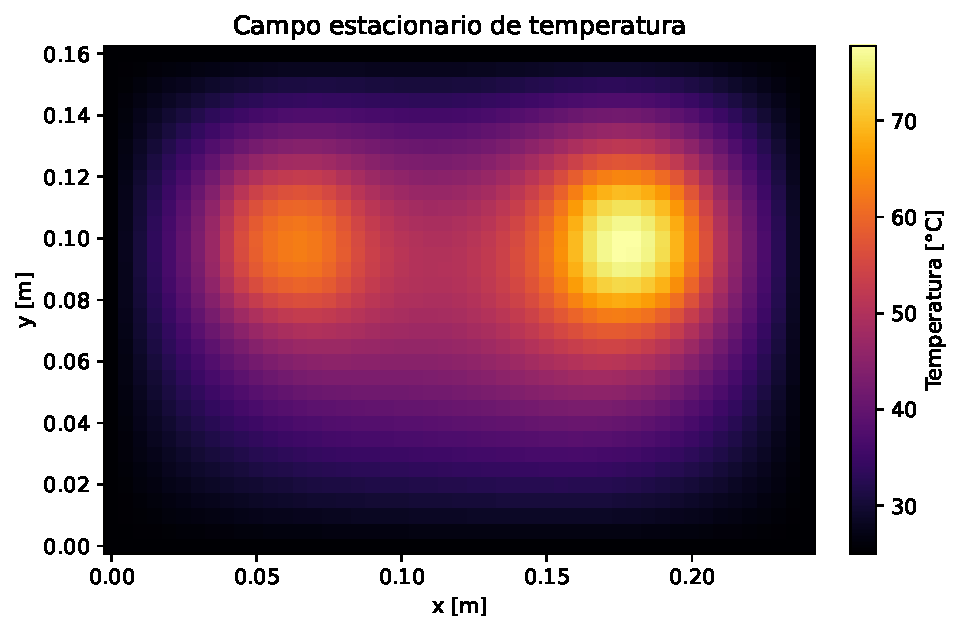
\includegraphics[width=\columnwidth]{../simulacion/figuras/02_mapa_termico.pdf}
\caption{Campo de temperatura estacionario del escenario base.}
\label{fig:mapa-termico}
\end{figure}

\begin{figure}[t]
\centering
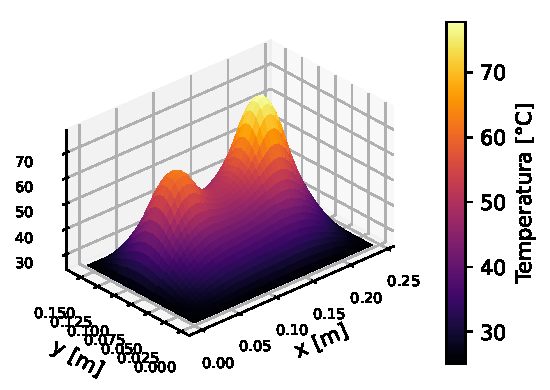
\includegraphics[width=\columnwidth]{../simulacion/figuras/03_superficie_3d.pdf}
\caption{Superficie del mismo campo estacionario presentado en la Figura~\ref{fig:mapa-termico}; la altura y el color representan la temperatura exportada por MATLAB.}
\label{fig:superficie-3d}
\end{figure}

\begin{figure*}[t]
\centering
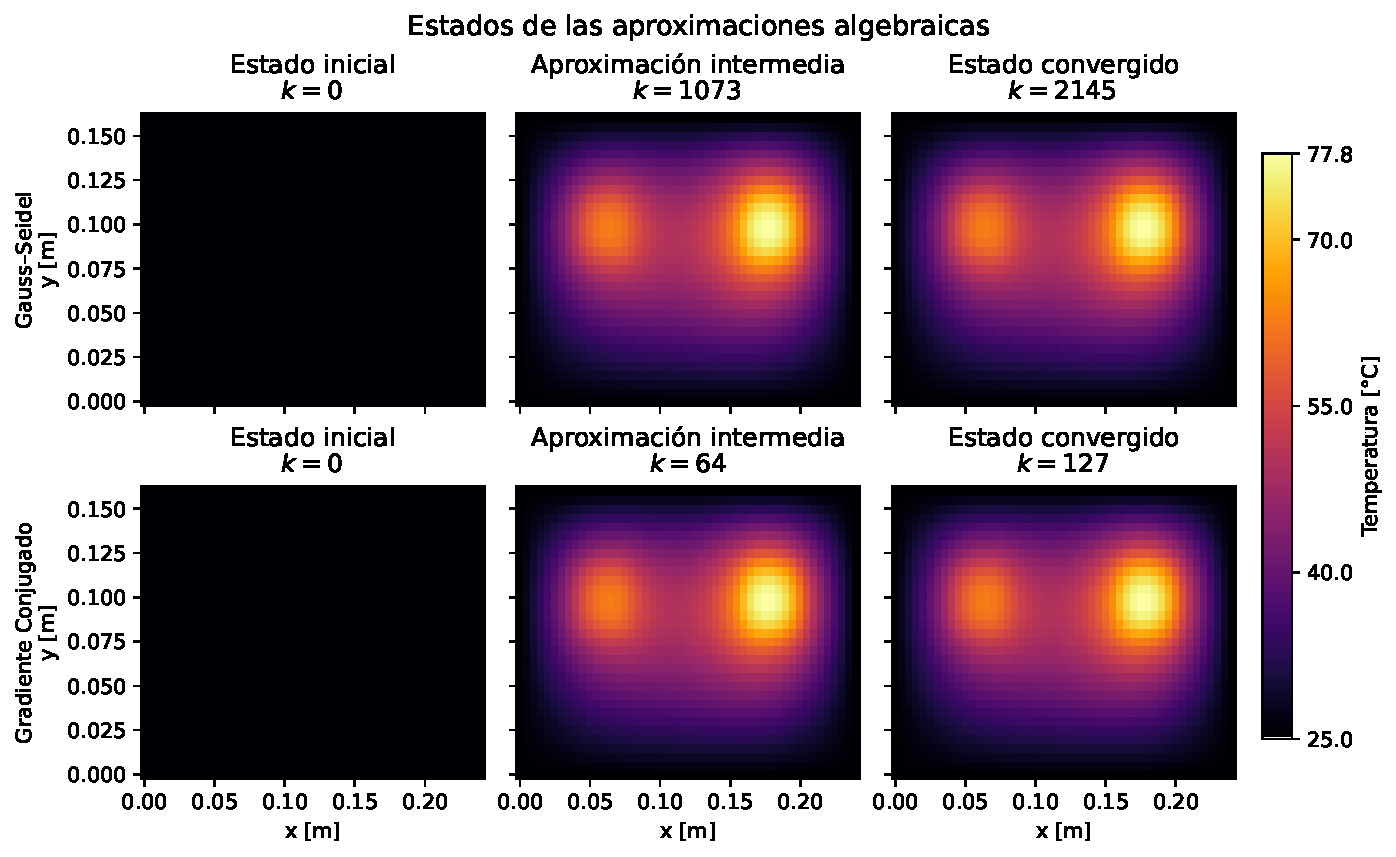
\includegraphics[width=0.94\textwidth]{../simulacion/figuras/04_evolucion_aproximaciones.pdf}
\caption{Estados inicial, intermedio y convergido de las aproximaciones algebraicas de Gauss--Seidel y Gradiente Conjugado. $k$ denota iteraciones del solucionador y no tiempo f\'isico; todos los paneles comparten la misma escala de temperatura.}
\label{fig:aproximaciones}
\end{figure*}

\begin{figure}[t]
\centering
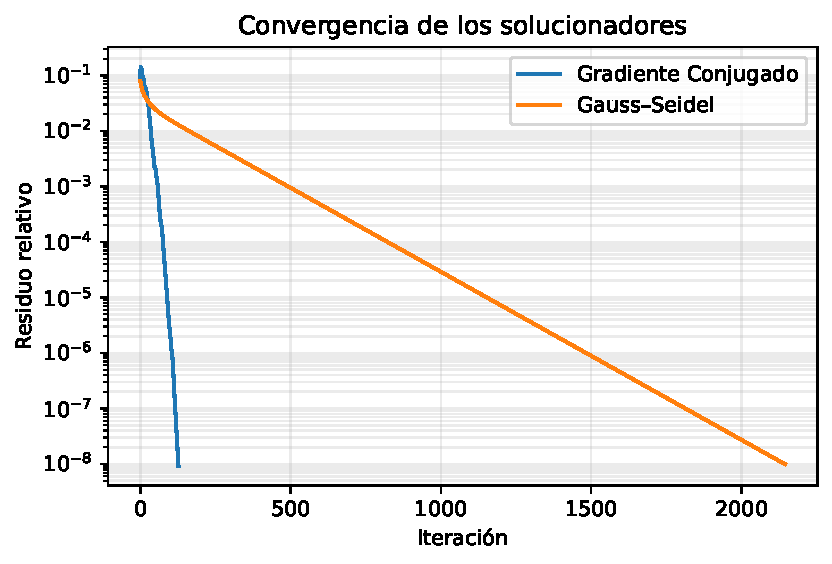
\includegraphics[width=\columnwidth]{../simulacion/figuras/06_residuo_iteraciones.pdf}
\caption{Residuo relativo frente a iteraciones en la malla base.}
\label{fig:residuos}
\end{figure}

\subsection{Refinamiento espacial (objetivo iii)}

Las ocho corridas iterativas de las cuatro mallas convergieron con residuo menor que $10^{-8}$. La Tabla~\ref{tab:refinamiento} muestra que la diferencia nodal m\'axima entre soluciones directas consecutivas se redujo de $0.2385$ a $0.06159$ y $0.01554\ ^\circ$C al duplicar la resoluci\'on. Esta reducci\'on observada es cercana a un factor de cuatro por refinamiento, consistente con el orden espacial esperado en este caso; la diferencia entre mallas no es un error exacto respecto de una soluci\'on anal\'itica. En la malla m\'as fina hay 24,257 inc\'ognitas y el m\'aximo directo es $78.03446\ ^\circ$C.

\begin{table}[t]
\centering
\begin{threeparttable}
\caption{Resultados directos del refinamiento de malla}
\label{tab:refinamiento}
\footnotesize
\begin{tabular}{rrrr}
\toprule
Malla & $N$ & $T_{\max}$ ($^\circ$C) & $\Delta T_m$ ($^\circ$C)\\
\midrule
$25\times17$ & 345 & 77.40879 & 0.23847\\
$49\times33$ & 1457 & 77.75924 & 0.06159\\
$97\times65$ & 5985 & 78.01291 & 0.01554\\
$193\times129$ & 24257 & 78.03440 & --\\
\bottomrule
\end{tabular}
\begin{tablenotes}\footnotesize
\item \textit{Nota.} La diferencia es el m\'aximo absoluto nodal entre la soluci\'on directa de esa malla y la interpolaci\'on bilineal de la siguiente malla m\'as fina. La malla m\'as fina no tiene comparador configurado.
\end{tablenotes}
\end{threeparttable}
\end{table}

En la malla de 24,257 inc\'ognitas, Gauss--Seidel requiri\'o 29,541 iteraciones y una mediana de 52.190 s (desviaci\'on est\'andar 5.502 s); CG requiri\'o 485 iteraciones y una mediana de 0.2043 s (desviaci\'on est\'andar 0.00526 s). La Figura~\ref{fig:costo} resume las medianas e intervalos intercuart\'ilicos de tres repeticiones por malla y m\'etodo. La variaci\'on entre ejecuciones y equipos aconseja interpretar estos cronometrajes como evidencia de la sesi\'on registrada, no como una raz\'on de rendimiento universal.

\begin{figure}[t]
\centering
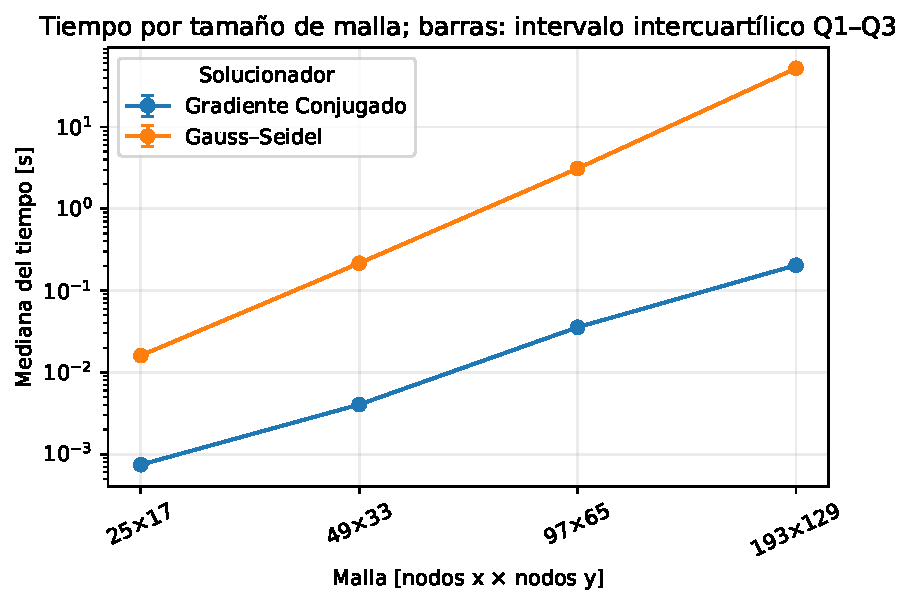
\includegraphics[width=\columnwidth]{../simulacion/figuras/07_costo_refinamiento.pdf}
\caption{Tiempo de soluci\'on por tama\~no de malla; escala vertical logar\'itmica.}
\label{fig:costo}
\end{figure}

\subsection{Sensibilidad de las fuentes (objetivo iii)}

Al variar CPU entre $0$ y $18$ W con GPU fija en $18$ W, $T_{\max}$ aument\'o de $75.0267$ a $79.2360\ ^\circ$C. Al variar GPU entre $0$ y $27$ W con CPU fija en $12$ W, el m\'aximo aument\'o de $58.3511$ a $102.6621\ ^\circ$C. En ambas series se mantuvieron los restantes par\'ametros. La Figura~\ref{fig:sensibilidad} resume los ocho casos y las ubicaciones de los puntos calientes exportadas por MATLAB.

\begin{figure}[t]
\centering
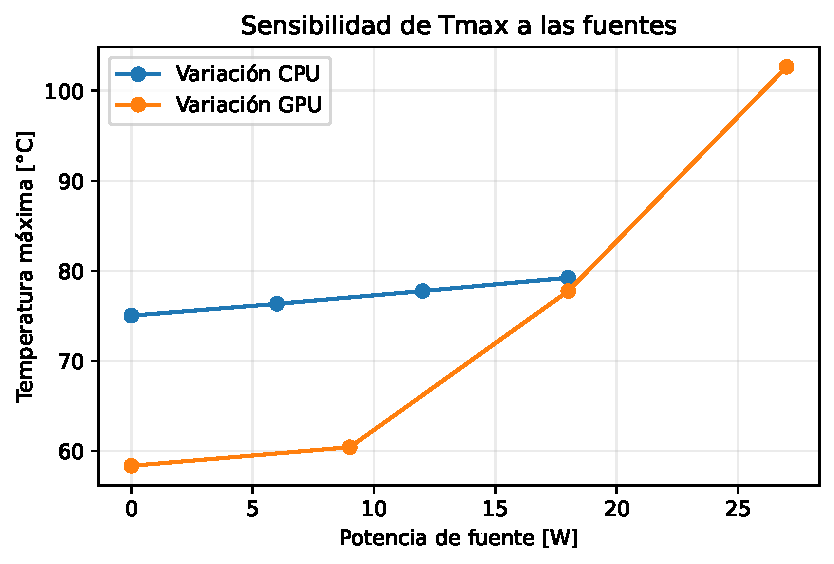
\includegraphics[width=\columnwidth]{../simulacion/figuras/08_sensibilidad_termica.pdf}
\caption{Sensibilidad del m\'aximo de temperatura a la potencia de CPU y GPU.}
\label{fig:sensibilidad}
\end{figure}

\subsection{Estr\'es num\'erico y validaci\'on (objetivos i y iv)}

Para las cuatro tolerancias solicitadas, ambos m\'etodos alcanzaron convergencia. A $10^{-12}$, Gauss--Seidel necesit\'o 3466 iteraciones y obtuvo residuo $9.99\times10^{-13}$; CG necesit\'o 162 iteraciones y obtuvo $8.98\times10^{-13}$. En las pruebas con fuentes multiplicadas por $1000$ y con potencia negativa de CPU, ambos m\'etodos tambi\'en terminaron con estado convergente y residuos menores que $10^{-8}$. El caso extremo y el no f\'isico se reportan solo como pruebas algebraicas, no como escenarios de una laptop. No se observ\'o fallo de convergencia en las corridas registradas.

La verificaci\'on MATLAB document\'o simetr\'ia relativa nula, factorizaci\'on de Cholesky exitosa, error m\'aximo de frontera igual a cero, balance de potencia de $12$ W y $18$ W, y error de linealidad de $4.26\times10^{-14}\ ^\circ$C. El control deliberado con una iteraci\'on m\'axima se identific\'o como \texttt{max\_iterations}; por ello, el estado de no convergencia se detect\'o. El reporte completo y las tablas de cada experimento se conservan en \texttt{simulacion/resultados/} y \texttt{simulacion/pruebas/}.
